\documentclass{article}

\usepackage[a4paper,left=18mm,right=18mm,top=20mm,bottom=18mm]{geometry}
\usepackage[italian]{babel}

\usepackage{titling}
\usepackage{graphicx}
\usepackage{subcaption}
\usepackage{float} 
\usepackage{hyperref}


\title{Documentation for Software engineering project}
\author{Nicolas Anselmi, David Guzman Piedrahita and Marco Vinciguerra}
 
\begin{document}
\maketitle        
\section{Project Plan}
\subsection{Introduction}
Il progetto prevede lo sviluppo di una mobile app per gestire la prenotazione di 
un negozio di parruccheria. C'è la possibilità di avere due tipi di utente:

 La novità di questo progetto consiste nel fatto che è un tipo di sistema P2P in cui un utente può essere contemporaneamente cliente
e (se vuole) gestore. Questo modello di business è fatto anche da Uber in cui un autista può essere sia cliente che autista.
\\Il target della clientela è market driven in quanto il core business dell'azienda si basa su percentuali delle transazioni.
Il cliente ha la possibilità di prenotare diversi 
tipi di acconciatura direttamente senza interfacciarsi /chiamare direttamente il proprietario
del negozio, usando invece tramite l'applicazione. Ogni tipologia di taglio selezionabile e può consentire una data customizzabile di prenotazione 
da parte del cliente. 
\\I membri del team sono: Nicolas Anselmi, David Guzman Piedrahita e Marco Vinciguerra.
   
\subsection{Process model}
Il life cycle del progetto è agile, in particolare la tecnica utilizzata è SCRUM con
sprint di circa 5 giorni. Inoltre viene utilizzato un triage per
gestire i compiti (MoSCoW).
\\Inoltre viene applicato un modello di prototipazione incrementale in cui ad ogni git viene aggiunto una funzionalità al sito e in più deve essere sempre disponibile
su Github una versione funzionante del progetto.
\\Per accelerare il processo di apprendimento viene applicato anche il processo di pair programming, 
pratica molto utilizzata nei metodi AGILE.
\\Per quanto riguarda i requirements si utilizza il Kano Model el il MoSCoW model.
Il periodo di sviluppo parte poco prima di Natale. Ogni giorno verso le 9 30 del mattino 
c'è un daily scrum tenuto dallo scrum master in cui si discutono le problematiche riscontrate durante 
il giorno precedente e le possibili soluzioni a queste.

\subsection{Organization of the project}
Il progetto, dovuto alla sua natura, deve intefacciarsi sia con utenti  che usufruiscono del servizio di prenotazione, sia da utenti che mettono a disposizioni i loro servizi commerciali.
Il team di sviluppo è composto dai succitati integranti. Per portare a termine l'applicazione, ci sono dei knowledge-gap che dovranno essere colmati tramite la lettura di documentazione e
l'uso di risorse online: particolarmente nel caso del framework Flutter per il frontend development.

\subsection{Standards, guidelines, procedures}
I principali linguaggi di programmazione del progetto sarà dart, quest'ultimo
viene esteso tramite flutter.
Si usano i coding standards di flutter.
\\Per gestire l'assegnazione e il corretto sviluppo si usa un template di Notion per gestire i compiti.
\\Gli IDE che vengono utilizzati sono: VSC e terminale con VIM.

\subsection{Management activities}
Ogni settimana viene fatto un report informale sui progressi in corso fatti dal team di sviluppo per avere un'idea sull'avanzamento del progetto.
\\Le modifiche critiche del progetto devono essere accettate dal CCB (a sua volta composto dall'intero team di sviluppo), le altre possono essere fatte 
liberamente.
\\Questi report, insieme alle decisioni definite negli scrum meeting, rappresentano la principale strategia per valutare velocemente lo status del progetto, e, 
di conseguenza, sono utili a fare course-correction.
\\Difatti, è proprio in questo modo che è previsto bilanciare l’equilibrio tra requirements e l’impegno necessario per soddisfarli.  
\subsection{Risks}
Il rischio principale è di non consegnare in tempo il progetto o di non consegnare un progetto perfettamente funzionante.
\subsection{Staffing}
I membri del team sono: Nicolas Anselmi, David Guzman Piedrahita e Marco Vinciguerra.
\\Per provare a vedere come funziona il mestiere il ruolo dello SCRUM master cambia a rotazione e si parte dalla settimana 
che inizia col 13 dicembre. Il primo SCRUM master sarà David, la settimana dopo Nicolas e quella dopo Marco Vinciguerra e così via...

\subsection{Methods and techiniques}
Per gestire gli sprint è stato utilizzato un template di Notion in quanto ha la possibilità di schedulare i task in base alla scadenza e in base ad un ordine gerarchico.
\\Per gestire la fase di testing si usa il tool better flutter tests che fa lui il testing sul framework Flutter. Il test viene scritto automaticamente dal tool e quindi 
non si applica fin da principio.
\\Per quanto riguarda la specifica dei requisiti si utilizza lo standard IEEE 830.
\\Si prevede l'uso di una strategia COTS per la scelta di diversi moduli o, più precisamente, widget di Flutter, che consentono di implementare velocemente
elementi UI classici, senza scrivergli da zero.
\\Per quanto riguarda i test di Dart si utilizza Dart unit testing e si utilizza il TDD e per garantire la continuos integration si usa Travis CI che partirà ad ogni 
Git e ogni 24 ore.
\\Per i database si utilizza Firebase  per creare e gestire il database delle prenotazioni.
\\La gestione delle modifiche viene svolta tenendo in conto le considerazione del punto 5 e, soprattutto, il punto 13.
\subsection{Quality assurance}
Per garantire la qualità del prodotto viene utilizzato lo standard ISO 9001.

\subsection{Work packages}
Alcuni dei sottoprogetti (work package) che sono stati definiti a priori.
\\ In viste della natura agile del progetto, questi work-package saranno estesi e modificati o evoluti nelle diverse iterazioni del life-cycle:
\begin{itemize}
    \item Fase di design di schemi UML
    \item Imparare ad utilizzare Flutter e dart
    \item Implementare l'applicazione con un'interfaccia grafica (front-end)
    \item Implementare la domain logic (back-end)
    \item Uso di un database
    \item Fare il testing sul prodotto
    \item Fare testing usando l'applicazioni in telefoni reali (non simulator)
\end{itemize}

\subsection{Resources}
Gli obiettivi di prototipazione proposti dal progetto in questione richiedono solo l'uso di computer adatti alla programmazione nei suddetti linguaggi e framework.
Dopo diverse iterazioni di prototipazione è prevista la possibilità di usare dei cloud-server che ricevano e gestiscano le richieste degli utenti tramite i loro client/app. 

\subsection{Budget and schedule}
Il tempo preventivato per il progetto è di circa 70 ore a testa, quindi in totale saranno richieste 210 ore.
\\La documentazione ha la priorità più alta, ma la necessità di imparare a utilizzare Flutter, di imparare a gestire UI per la prima volta, rappresentarà comunque un alto costo in termini di tempo.
\subsection{Changes}
Col tempo potrebbero cambiare le richieste da parte del cliente durante la fase di validazione di ogni processo.
\\Al supporto delle attività di change management vengono utilizzati i due tool usati anche per altri aspetti del progetto, ovvero: 
\\Github, che in questo caso funge da piattaforma per accettare o rifiutare le modifiche version-oriented e per consentire di usare il forked develpment; 
\\e Notion che, non essendo un tool specifico per lo sviluppo, serve invece a gestire l’organizzazione delle tempistiche e dei sotto-progetti a un livello di astrazione più alto.
\\I contenuti di questi tool, e i diversi report dei punti precedenti, servono come guida per la compilazione di un eventuale configuration management plan che conterrà una management section e activities. I documenti generati come risultato del punto 5 sono particolarmente utili per la management section.

\subsection{Delivery}
Il project plan verrà consegnato entro il 27 dicembre 2021
\\La consegna verrà fatta 5 giorni prima dell'esame orale.
\newpage
\section{Scrum life cycle}
Il life cyle utilizzato è Scrum. Di conseguenza, saranno usate iterazioni con limiti di tempo predefinito, i cosiddetti sprint. La loro composizione e quantità è soggetta a modifiche.
La durata tradizionale degli sprint e di 2 a 4 settimane, ma in questo caso si utilizzano sprint di durata da 5 a 10 giorni per velocizzare il processo.
\\Pre cercare di capire come funzionano i ruoli all'interno di Scrum, essi vengono cambiati a rotazione settimanale.

\subsubsection{Product owner} è l'intermediario tra cliente e dipendenti e solitamente si occupa lui di gestire il backlog. In questo 
caso non c'è nessuno che si occupa di gestire l'interazione col cliente.
\subsubsection{Development team} è il team che si occuopa di sviluppare il progetto. Quando si fa questo ruolo
ci si occupa di svolgere i ruoli che sono inseriti nel backlog.
\subsubsection{ScrumMaster} Quando uno degli elementi del gruppo diventa ScrumMaster
si occupa di aiutare a risolvere i problemi del development team tramite consigli.


\subsection{Sprints} 
\subsubsection{State of the backlog}
il backlog iniziale si basa completamente sui requisiti che sono disponibile nel corrispettivo documento, nella fase di architettura il backlog tiene considerazione dei suddetti requisiti ma anche del contesto architettonico (vedi documento architettura) . 
\subsection{Sprint 1}
\begin{itemize}
    \item Creazione della prima parte della UI
    \item Informarsi sul funzionamento dei database in flutter
    \item Proseguire con la documentazione
    \item Informarsi sul testing
    \item Unit testing
\end{itemize}
\subsection{Sprint 2}
\begin{itemize}
    \item Avanzamento della UI
    \item Implementazione dell'interfaccia di Login
    \item Iniziare il testing
    \item Implementazione di un database relazionale
    \item Proseguire con la documentazione
    \item Widget testing
\end{itemize}
\subsection{Sprint 3}
\begin{itemize}
    \item Perfionamento della UI
    \item Implementazione di un real time database
    \item Mappare l'interfaccia di Login col database
    \item Proseguire con la documentazione 
    \item Continuos integration con Travis per il testinf
\end{itemize}
\subsection{Sprint 4: database - experiments}
\begin{itemize}
    \item Perfezionamento del tema e delle migliore tecniche
    \item Build per l'interfaccia web
    \item Fine della documetnazione
   
\end{itemize}
\begin{itemize}
\item Sprint planning meeting 
\\26/12/21 
\\Sono stati definiti gli obiettivi base del progetto e dello sprint. Dal backlog (e, a sua volta, dai requirements) sono stati scelti i seguenti elementi per lo sprint backlog:
\\-	Creazione della documentazione dei requirements.
\\-	Creazione della documentazione di architettura.
\\-	Proposte iniziali di schemi UML (soggetti a molte modifiche dovuto al seguente punto).
\\-	Precisazione delle librerie e framework elements da usare per l’implementazione software.
\\-	Processo cots per la scelta delle suddette librerie e altri elementi di framework.

\item Report degli Scrum meeting più significativi
\\28/12/21 
\\Discussione sui primi schemi UML. Proposte per migliorarli e modificarli + Backlog refinement
\\30/12/21
\\Discussione su come gestire nel modo più efficiente la costruzione della UI + Backlog refinement
\\2/1/22
\\Discussione di diversi elementi modulari UI trovati nei giorni precedenti e che erano candidati per uso come UI ufficiale. 
\\5/1/22
\\Discussione sul come costruire la home page dell’applicazione + Retrospective meeting notes
\\6/1/22
\\Cross-review dei diversi file di documentazione creati (requirements, architecture, testing, ecc) 
\\12/1/22
\\Scrum per gestire la UI
\\15/1/22
\\Scrum per discutere lato backend e Firebase, abbandonata l'idea di usare un database relazionale classico
\\18/1/22
\\Discussione su come utilizzare Firebase
\\21/1/22
\\Implementazione di Firebase + Sprint review meeting 
\\24/1/22
\\Prova generale dell'applicazione
\\27/1//22
\\Discussione e revisione della documentazione + Retrospective meeting notes

\end{itemize}
\newpage
\section{People Management and Team Organization}
La suddivisione e il funzionamento dello Scrum team è citato al paragrafo precedente. 
\\Il team è formato da 3 persone e la comunicazione avviene tramite chiamate telefoniche.
\\Come approccio di organizzazione si usa l'approccio di Mintzberg, i punti principali sono:
NON SO COSA SCRIVERE
\begin{itemize}
     \item \textbf{simple structure}: Non c'è una persona del gruppo che comanda ma c'è un livello paritetico
        e la comunicazione è veloce e diretta
    \item \textbf{Machine bureaucracy}: Una volta stabiliti gli output non si interviene sull'andamento dei membri
    del team ma l'importante è raggiungere gli obiettivi
    \item \textbf{Divisionalized form}: La standardizzazione del processo produttivo la si ha
    gli standard di qualità del codice di flutter
    \item \textbf{Professional bureaucracy}: Non c'è formalità e nessun tipo di gerarchia
    \item \textbf{Adhocracy}: Tutti i componenti si occupano di fare un po' tutti i ruoli per 
        quanto riguarda lo sviluppo del software, la gestione del database e dei casi di test
    
\end{itemize}
   \newpage
\section{Software Quality}
\subsubsection{CMM}
Per quanto riguarda il CMM (Capaibility Maturity Model) esistono 5 livelli di maturità del software, essi sono:
\begin{itemize}
    \item Initial 
    \item Repeatable
    \item Defined
    \item Quantitatively managed
    \item Optimizing
\end{itemize}
In questo progetto si punta ad utilizzare il terzo livello 3 (Defined) in cui ogni attività viene documentata
e standardadizzata per l'intera organizzazione per quanto riguarda il  processo per il design, development, testing e via dicendo.

\subsubsection{ISO 9216}
Per quanto riguarda la product conformance si fa riferimento al seguente link: \url{https://www.geeksforgeeks.org/iso-iec-9126-in-software-engineering/}
\\Esso si basa sui 4 seguenti principi:
\begin{itemize}
    \item \textbf{Part 1: "Quality model"} 
    \item \textbf{Part 2: "External metrics"} 
    \item \textbf{Part 3: "Internal metrics"} 
    \item \textbf{Part 4: "Quality in use metrics"} 
\end{itemize}
Per chiarire meglio il concetto si fa riferimento al seguente grafico:
\\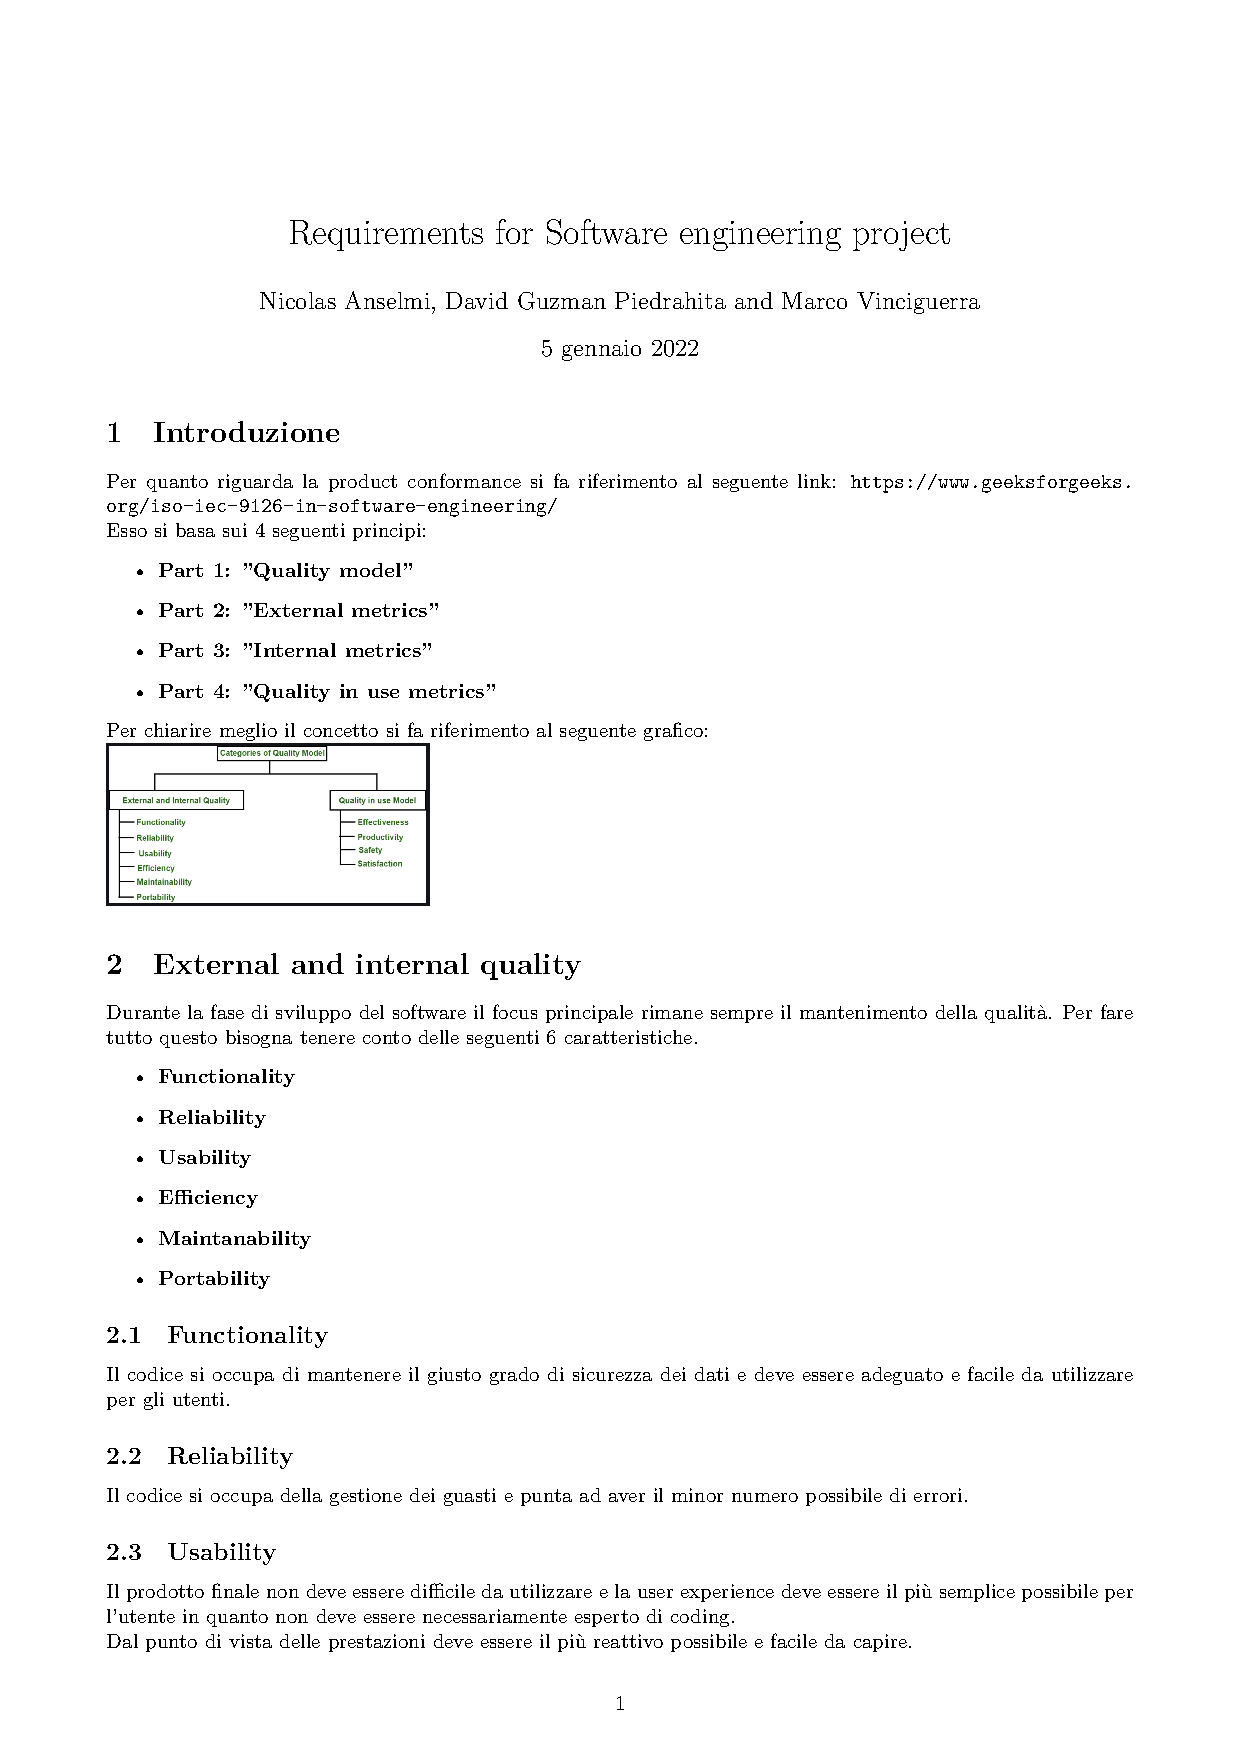
\includegraphics[scale = 0.25]{"Immagini/ISO9126.PNG"}
\subsection{External and internal quality}
Durante la fase di sviluppo del software il focus principale rimane sempre il mantenimento della qualità.
Per fare tutto questo bisogna tenere conto delle seguenti 6 caratteristiche.
\begin{itemize}
    \item \textbf{Functionality} 
    \item \textbf{Reliability} 
    \item \textbf{Usability} 
    \item \textbf{Efficiency} 
    \item \textbf{Maintanability} 
    \item \textbf{Portability} 
\end{itemize}

\subsubsection{Functionality}
Il codice si occupa di mantenere il giusto grado di sicurezza dei dati e deve essere adeguato e facile
da utilizzare per gli utenti.

\subsubsection{Reliability}
Il codice si occupa della gestione dei guasti e punta ad aver il minor numero possibile di errori.

\subsubsection{Usability}
Il prodotto finale non deve essere difficile da utilizzare e la user experience deve essere il più
semplice possibile per l'utente in quanto non deve essere necessariamente esperto di coding.
Ad esempio i bottoni sono studiati per essere il più semplici e intuitivi possibile.
\\Dal punto di vista delle prestazioni deve essere il più reattivo possibile e facile da capire.

\subsubsection{Efficiency}
Si vuole creare il programma più efficiente possibile che utilizzi il minimo delle risorse del dispositivo
da cui si utilizza l'applicazione. 
\\Per migliorare l'efficienza si è usato per esempio la variabile const nella UI.

\subsubsection{Maintanability}
Il codice deve essere scritto nel modo più conforme alle regole di standard di programmazione per favorire
la leggibilità e la successiva manutenzione.

\subsubsection{Portability}
Il programma deve funziona su più piattaforme possibilili, Flutter permette con un solo codice 
sorgente di scrivere programmi per più piattaforme.

\subsubsection{Security}
I dati vengono criptati tramite la piattaforma encrypt.
\subsection{Quality in use Model}
Si basa sulle seguenti 4 caratteristiche che si vuole soddisfare:
\begin{itemize}
    \item Effectiveness
    \item Productivity
    \item Safety
    \item Satisfaction 
\end{itemize}

\subsection{Introduzione alla Taxonomy quality}
Questo file si occupa del descrivere i requisiti tassonomici di qualità del progetto.
\\Per quanto riguarda la definizione di McCall.
\\In particolare si vuole utiizare i seguenti driver/linee guifa per la produzione, revisione e
transizione  del codice.     
\subsection{Product operation}
\begin{itemize}
    \item Correctness: se il sistema fa quello richiesto
    \item Reliability: se il sistema è abbastanza accurato
    \item Efficiency: se il sistema utilizza l'hardware efficientemente
    \item Integrity: se il sistema è sicuro
    \item Usability: se il sistema è utilizzabile
\end{itemize}
In particolare ci si sofferma sull'usability, correctness e reliability in quanto il 
prodotto deve funzionare il meglio possibile.

\subsection{Product revision}
\begin{itemize}
    \item Maintainability: se il sistema in caso di guasto è riparabile
    \item Testability: se il sistema è testabile 
    \item Flexibility: se il sistema è facilmente cambiabile
\end{itemize}
Il prodotto che si sta costruendo in questo caso tende a essere molto testabile in 
quanto i test per verificare la correttezza vengono creati ed eseguiti poco dopo la  creazione
delle classi.

\subsection{Product transition}
\begin{itemize}
    \item Portability: se il software è utilizzabile su altre piattaforme
    \item Reusability: se il software è riutilizzabile
    \item Interoperability: se il sistema è interfacciabile con altri sistemi
\end{itemize}
Il sistema tenderà a essere molto portabile in quanto è stato fatto con Flutter, il quale
tende ad essere molto scalabile.

\subsection{Qualità per il codice in Dart}
Per il codice in Dart è stato implementato il Dart Analyzer, che si ottiene modificando il file
$analysis_options.yaml$ e tramite il comando da terminale dart analyze si fa un test per 
vedere se le qualità prese in considerazione sono valide e rispettate.
\\La documentazione necessaria per informarsi su questo tipo di standard è stata presa
dal seguente link: \url{https://pub.dev/packages/analyzer}.
\\Alcuni tra i parametri presi in considerazione per garantire la qualità sono:

\begin{itemize}
    \item Maximum nesting level
    \item Ciclomatic complexity
    \item Number of parameters
    \item Source lines of code
\end{itemize}
Per usare i quality metrics si usano i segueti comandi digitati da terminale:
\begin{itemize}
    \item Miglioramento delle performance del codice: dart$\_$analyze
    \item Calcolo complessità: flutter pub run dart$\_$code$\_$metrics:metrics analyze lib
    \item File non utilizzati: flutter pub run dart$\_$code$\_$metrics:metrics check-unused-files lib
\end{itemize}

La configurazione è presente nel file analysis\_options.yaml.
\\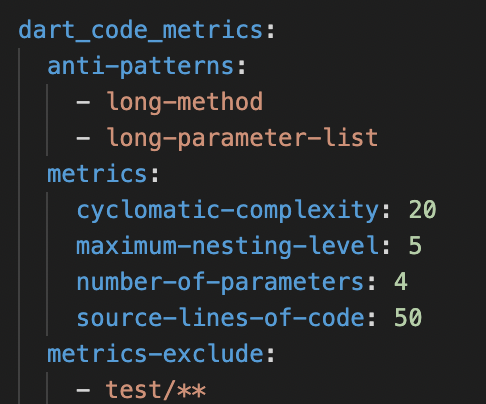
\includegraphics[scale = 0.5]{"Immagini/ParametriQuality.png"}

Ecco un esempio di output di un test fatto con dart analyze:
\\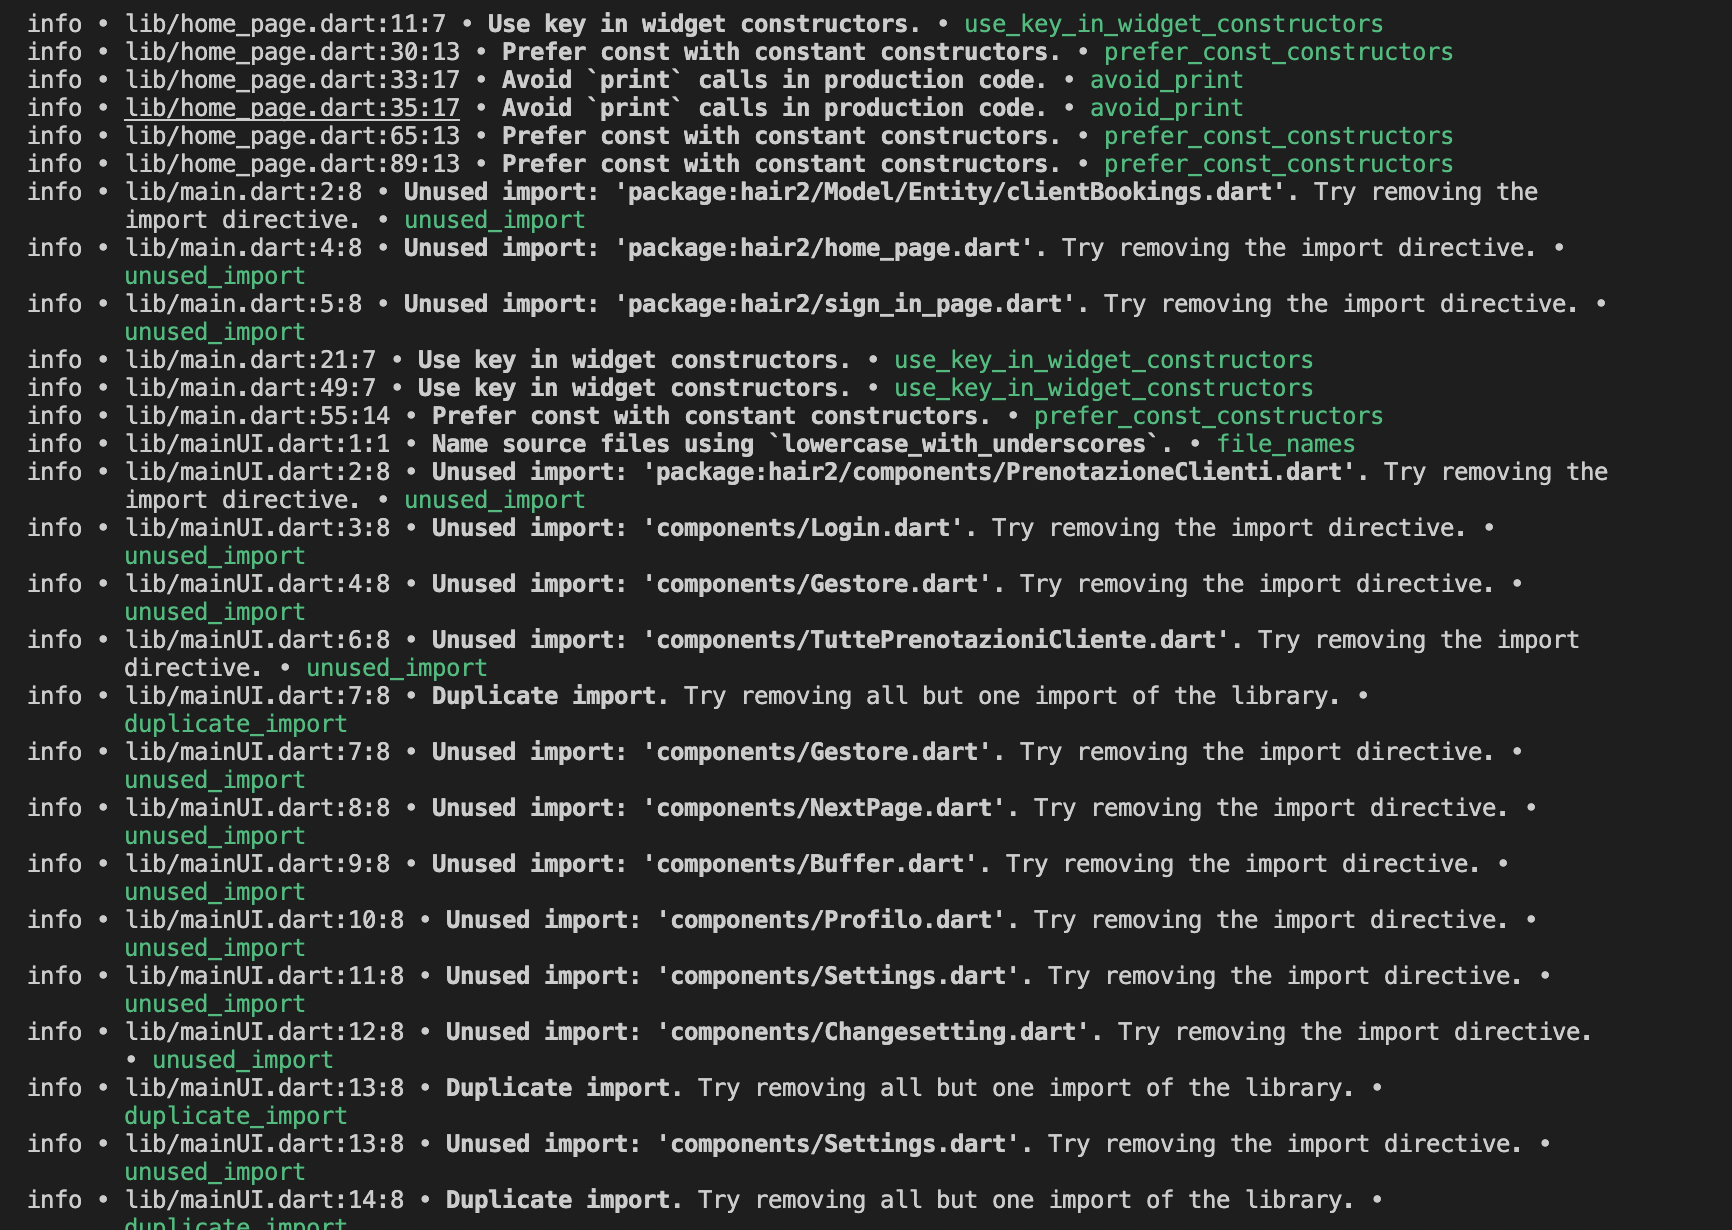
\includegraphics[scale = 0.5]{"Immagini/Dart_analyze.png"}
\\Col tempo questi consigli sono diminuiti di circa l'80 \% e il 20\% riguarda istruzioni
che sono deprecated ma che sono necessarie per il progetto.
\\Per migliorare l'efficienza si è usato per esempio la variabile const nella UI che toglie un errore in dart\_analyze.

\newpage
\section{Requirement Engeneering-IEE830}
\subsection{Purpose} 
Questo documento segue la struttura proposta dallo standard IEEE 830 per la definizione dei requirements. Questi rappresenta uno dei criteri fondamentali per valutare l’adeguatezza dell’implementazione ottenuta nei diversi sprint e un punto di partenza per le seguenti fasi dello sviluppo dell’applicazione.
\subsection{Scope}
L’obiettivo centrale è costruire un’applicazione per la gestione di prenotazioni di tagli in saloni di bellezza, eventualmente estendibile ad altri servizi. 
\\In grandi linee, l’applicazione dovrebbe consentire di facilitare il processo della creazione di appuntamenti, evitando l’uso di chiamate, sostituendole con procedure online molto più veloci e friction-less. 
\\L’interfacciamento dell’utente con l’applicazione deve essere tale che, nonostante la più alta complessità inerente a una soluzione model-view-controller rispetto all’uso di semplici chiamate, l’utilizzatore percepisca un netto miglioramento rispetto al solito modo di fare e a prescindere delle loro conoscenze informatiche. 
\\Di conseguenza, l’applicazione non solo deve offrire la funzionalità centrale delle prenotazioni, ma in più deve farlo in un modo intuitivo. 

\subsection {Definitions, acronyms and abbreviations }
\subsection {References} 
\subsection {Overview} 
Dopo questa introduzione, il documento è composto da due ulteriori fasi: la parte 2, che da una descrizione globale dei requirements, e la parte 3, che elenca e classifica tutti i diversi requirements individuali, usando il modello Kano e Moscow.
\subsection {Overall description} 
\subsection {Product perspective} 
Non ci sono database o altre strutture informatiche preesistenti, in quanto il pubblico di destinazione è composto proprio da saloni di bellezza che gestiscono le loro prenotazioni in modo informale. La costruzione del software deve dunque partire da zero.
\\ Per la fase di elicitation sono state usate le strategie di open-ended interview, task analysis derivante anche da esperienze personali e natural language descriptions. 
\\ Le successive fasi di V and V e di negotiation saranno svolte dopo la generazione di un primo prototipo.
\subsection {Product functions} 
A continuazione sono elencati le funzionalità centrali, l’elenco dei requirements a una granularità più precisa sono disponibili nella parte 3.
\begin{itemize}
    \item Possibilità di prenotare tagli e, eventualmente, altri servizi offerti dai saloni.
    \item Possibilità di visualizzare le prenotazioni future e passate associate al salone in questione.
    \item Possibilità di tener traccia dei clienti con degli appositi profili utente/cliente associati a informazioni rilevanti.
    \item Disponibilità di visualizzare l’andamento dei ricavi risultanti dalle prenotazioni. 
\end{itemize}
\subsection {User characteristics} 
Come detto sopra, il prodotto deve essere costruito per soddisfare le esigenze di un pubblico di destinazione con conoscenze tecniche basilari (uso di smartphone e applicazioni user-friendly). 
\\L’UI dell’applicazione deve essere facile da usare da utenti ormai familiarizzatisi con altre applicazioni molto popolari (YouTube, Instagram…), di conseguenza il design-language deve essere coerente con quello al quale i potenziali utenti si sono ormai abituati, riducendo, di conseguenza, la learning-curve per usare il softwarele
\subsection {Constraints} 
Nella sua versione finale, l’applicazione dovrebbe essere utilizzabile sia da cliente che prenotano che da gestori di saloni di bellezza. 
\\I clienti dei saloni non devono avere accesso a informazioni del salone, come le prenotazioni di altri utenti, o i ricavi del salone. Dall’altro canto, i gestori non possono modificare certe informazioni dei profili degli utenti, ma possono modificare dati associati alle prenotazioni. 
\\Per il prototyping iniziale, si deve dare priorità alle funzionalità offerte ai gestori. L’implementazione delle prenotazioni remote fatte direttamente dagli utenti ha una priorità secondaria nelle prime fasi.
\subsection {Assumptions and dependencies} I sistemi usati sono: Firebase + Flutter login.
\subsection {Requisiti non funzionali} 
Il sistema deve avere un tempo di risposta minimo, velocità di utilizzo, dati accessibili solo
agli utenti specifici e quindi i seguenti requisiti non funzionali:
\begin{itemize}
    \item Prestazioni
    \item Sicurezza
    \item Manutenibilità
    \item Usabilità
    \item Affidabilità
    \item Disponibilità
\end{itemize}

\subsection {Specific requirements}
tra parentesi va scritta la priorità nel seguente modo: (Kano, Moscow)
\begin{itemize}
\item Possibilità di scegliere i diversi tipi di acconciature e in 
base al tipo di acconciatura scegliere la durata della prenotazione (Attactive, Must have)
\item Possibilità di registrarsi per la prima volta al sito da parte di un cliente. (Must-be, should have)
\item Utilizzo di un database per la gestione dei clienti. In alternativa si potrebbero utilizzare 
variabili per gestire le prenotazioni. (Must-be, should have)
\item Creazione di un profilo base utente per le prenotazioni. (Must-be, should have)
\item Che il sistema dellle prenotazioni non funzioni correttamente 
e che si accavallino sulla stessa fascia oraria. (One-Dimensional, should have)
\item Possibilità di mettere recensioni da parte dell'utente. (Questionable, could have).

\end{itemize}
\newpage 
\section{Software Architecture}
\subsection{Architecture design metod }
Per derivare una prima architettura funzionante partendo dai requirements specificati nell’apposito documento, si segue il criterio Generalized Model di Hofmeister et al. (2007).
\\Questo architecture design method è particolarmente utile per il progetto in questione, in quanto è strutturato utilizzando la terminologia e i ragionamenti di SCRUM, che è il life-cycle agile usato per l’applicazione e il suo sviluppo. 
\\In particolare, usa lo stesso concetto di backlog per elencare i diversi problemi che devono essere gestiti, e da esso è possibile scegliere gli elementi ritenuti più importanti in ogni particolare iterazione. 
\\Il backlog ha in input i requirements del progetto, con particolare attenzione ai requisiti di qualità; il contesto, che contiene idee aggiuntive sul come implementare un sistema che soddisfi i requisiti e, infine, i risultati della valutazione dell’architettura dell’iterazione precedente. 
\\Nel progetto verranno presi in considerazioni questi tre fattori per determinare le scelte di design. 
\\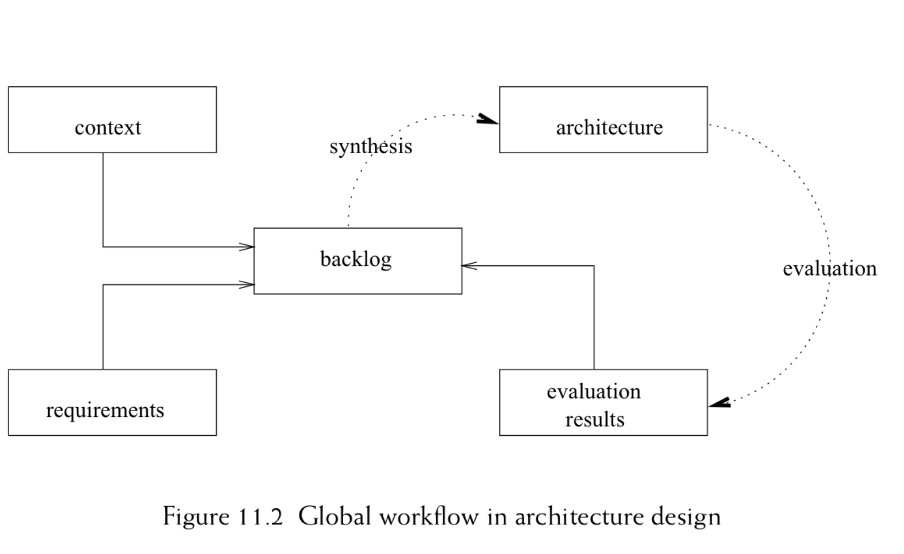
\includegraphics[scale = 0.75]{"Immagini/GeneralizedModel.png"}
\subsection{Decisioni di design} 
\subsubsection{Decision 1}
\begin{itemize}
\item Issue 
\item Decision
\item Status 
\item Assumptions
\item Alternatives
\item Rationale
\item Implications    
\item Notes
\end{itemize}
E' stato creato nei diagrammi UML diverse versioni dello stesso tipo di diagramma a seconda dello stakeholder
con cui ci si sta confrontando.
\\Il diagramma dei componenti e dei connettori risulta il seguente:
\\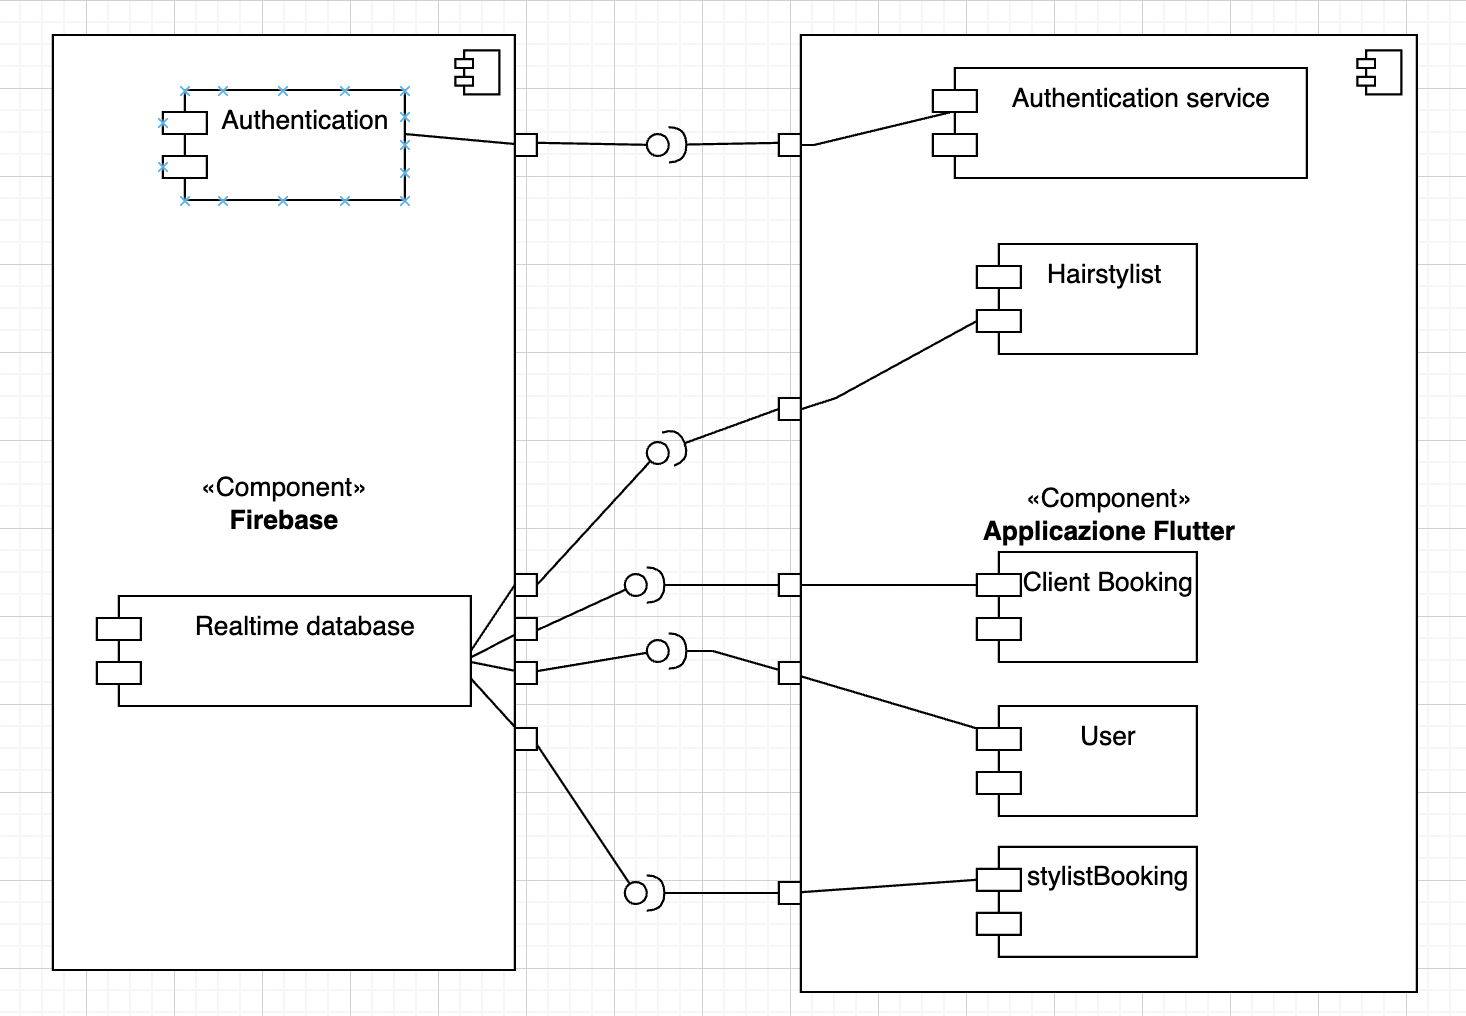
\includegraphics[scale = 0.45]{"Immagini/SoftArch.png"}
\subsection{Stile di architettura}
Lo stile architetturale dell’applicazione può essere assimilabile al repository style, in quanto ci sono due blocchi fondamentali: i client, composti del codice Dart/Flutter e disponibile come applicativo mobile, e il database, implementato usando i servizi non relazionali di Firebase Realtime Database offerti da Google. 
\\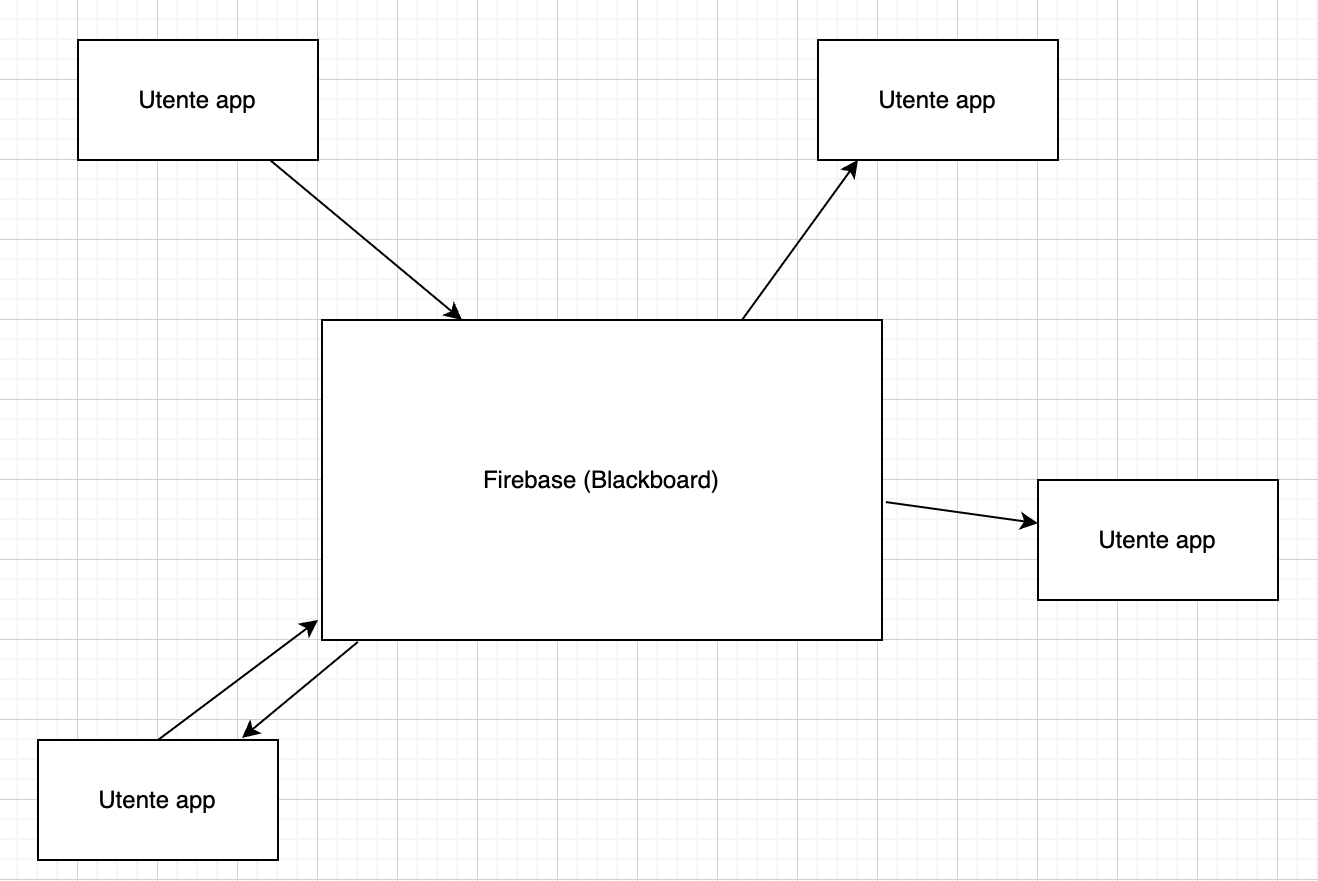
\includegraphics[scale = 0.45]{"Immagini/Blackboard.PNG"} 
\\Distinguiamo quindi come:
\begin{itemize}
\item System model: un sistema centralizzato di informazione strutturata che deve essere disponibile in scrittura e lettura per i diversi client, che sono invece gli elementi computazionali che sono indipendenti da esso.  
\item Components: si tratta di un unico componente memory (il database) e una quantità indefinita di client (a seconda del quantitativo di utenti) che sono invece dei component di tipo manager, in quanto mantengo, per un certo periodo di tempo, informazioni di stato e offrono diverse operation o funzionalità.
\item Connectors: chiamate sincrone e asincrone http tramite il web per contattare Firebase, comunicando tramite file json.  
\end{itemize}
Se, in più, teniamo in considerazione il ruolo centrale dei servizi offerti da Firebase, i quali non si limitano soltanto al database ma anche alle funzionalità di login e authentication gestite separatamente, possiamo definire l’architettura dell’app come una a servizi.
\\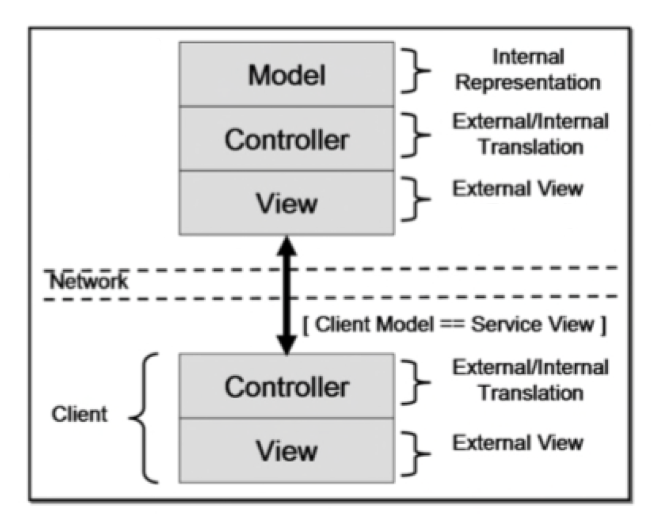
\includegraphics[scale = 0.45]{"Immagini/controllerViewArch.png"}
\\Dove si segue un modello basato sul classico model-view-controller, ma dove il model del client, al posto di essere implementato e gestito in locale, si appoggia a servizi esterni e standardizzati. 
\begin{itemize}
    \item Controller: il controller, a differenza del model, è implementato come parte del client vero e proprio, ed è stato costruito riflettendo, per quanto possibile, le diverse entità del mondo reale che interagiscono con l’applicazione o che rappresentano tipologie di dati pertinenti. La sua composizione e descritta per esteso nel class diagram.
    \item View: interamente costruita utilizzando i servizi offerti dal framework flutter, dove tutti i diversi tasti e pagine sono rappresentate da cosiddetti widget, che a usa volta sono delle classi dart. Dovuto all’elevato numero di classi che ne risulta e considerando che sono perlopiù assenti di metodi e campi nel senso tradizionale, non sono stati rappresentati nel class diagram. 
    \end{itemize}
\subsection{Rappresentazione architettura con IEEE 1471} 
Le rappresentazioni più concrete dell'architettura dell'applicativo vengono descritte attraverso degli schemi UML. Questi possono essere categorizzati come delle View indirizzate a diversi Stakeholder e definite tramite diversi Viewpoint, come formalizzato dallo standard IEEE 1471.
\\In particolare, i Viewpoint utilizzati per definire le View sono stati scelti tra quelli proposti da Bass et al. (2003).
\subsubsection{Module View}
I Viewpoint nella categoria module costituiscono una rappresentazione statica del sistema. Per questo progetto la module view più importante è Class. 
\\Le view costruite seguendo le specifiche del viewpoint Class descrivono il sistema in termini delle relazioni di eredità degli elementi. Il class diagram UML del progetto mette a disposizione questa informazione, assieme ad altre precisazioni dovute alla natura object-oriented del linguaggio di programmazione. 
\\\textbf{Add image}
\subsubsection{Component and connector View}
Il tipo di viewpoint scelto in questa categoria è il process viewpoint. Questo definisce il sistema in termini di comunicazione e sincronizzazione di processi. 
\\Come tutti gli altri viewpoint in questa categoria, offre una descrizione dinamica del software e, nel caso particolare del process viewpoint, è particolarmente utile per valutare performance e availability del sistema. 
\\In termini di UML, questa informazione è disponibile principalmente tramite il Sequence diagram. Questo schema spiega come i diversi elementi (classi) del sistema comunicano tra di loro attraverso procedure calls \textbf{(di tipo sincrono e asincrono)}.
\\Il component è la memory, il connector è la memory (database).
\subsubsection{Allocation View}
Questa categoria di viewpoint descrive la relazione tra il sistema e il mondo che lo circonda. Di conseguenza, può essere utilizzato per definire come viene assegnato hardware al software o come quest’ultimo viene mappato al file system. 
\\Per il progetto in questione, questo tipo di problematiche vengono gestite automaticamente dai framework utilizzati e quindi non sono competenza degli stakeholder che altrimenti ne farebbe uso, come i programmatori e i maintaner.
\\I viewpoint di tipo work assignment potrebbero essere utile per rappresentare graficamente la distribuzione del lavoro, ma in questo sprint vengono saltati per brevità. 
\newpage
\section{Software Design}
Per i parametri di qualità di design si utilizzano le seguenti metriche:
\\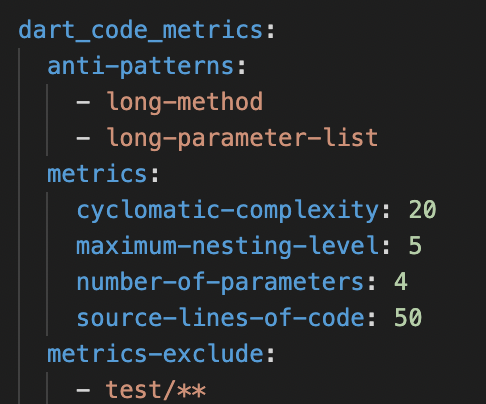
\includegraphics[scale = 0.75]{"Immagini/ParametriQuality.png"}
\\Invece per quanto riguarda i design pattern si utilizzano il Singleton, la Factory e il provider .
\subsection{Funzionamento delle classi Dart, in conformità con i requisiti funzionali e non:}
Come evidenziato dall’UML Class Diagram, le classi che si interfacciano con i servizi di Firebase sono state modellate partendo da entità del mondo reale, rappresentando quindi diversi ruoli e azioni previste nell’utilizzo dell’app. 
\\In particolare, un fattore che ha guidato il loro design è stata la necessità di gestire dati che non sono disponibili in locale con altri che invece lo sono. Tutto questo deve essere invisibile dal punto di vista dell’utente, usando delle loading screen nel caso peggiore. 
\\Di conseguenza, le classi che raggruppano informazioni disponibili nel database sono tutte munite da un collegamento diretto a esso tramite un attributo che è un oggetto speciale offerto dalle librerie di Firebase.
\\Ad esempio, la classe HairStylists, che ha il compito di essere un registro di tutti i parrucchieri che offrono i loro servizi ad ogni singolo istante, ha il campo privato db di tipo FirebaseDatabase, che di default viene inizializzato con l’oggetto che consente alla classe di comunicare con il database a un alto livello di astrazione. In più questa classe ha una particolarità: per consentire di avere un elenco di parrucchieri dinamico, e che quindi si tiene costantemente aggiornato rispetto al database, la classe conta con un metodo StreamChanges, eseguito nel costruttore, che crea una Subscription al database, dove la classe diventa un listener di tutte le modifiche del sotto-albero del json che contiene l’informazione pertinente.
\\In alternativa, è stato i implemento il metodo ReadStylists, che legge il contenuto del database un’unica volta, e quindi senza creare una Subscription; non è in uso nell’implementazione più recente, ma resta disponibile qualora ci fossero problematiche nel funzionamento di StreamChanges. 
\\ 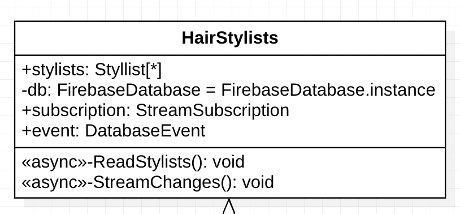
\includegraphics{Immagini/CalsseHairStylists.png} 
\subsection{Uso di strategie standard del linguaggio Dart e il Framework Flutter:}
\begin{itemize}
    \item -	Provider: usare flutter implica che l’interfaccia grafica è strutturata come un albero di ‘widget’, ovvero tasti e altri elementi interattivi. Spesso è necessario propagare informazione che è stata ottenuta in un punto dell’albero ad altri punti dell’albero (e.g quando si passa da una schermata alla prossima), pertanto esistono diverse strategie soddisfare questa necessità. 
    \\Per questo progetto, si usano i cosiddetti Provider, i quali sono la migliore alternativa perché consentono di rendere oggetti che sono in un nodo dell’albero raggiungibili per tutti i suoi figli (al posto di solo passare dei parametri, e di dover fare il hard-coding di questo passaggio di parametri in ogni transizione di nodo a nodo). Le classi che ne fanno uso devono estendere la classe ChangeNotifier, e questo è proprio il caso delle summenzionate classi che contattano il database, in quanto i loro dati possono essere necessari in diversi punti dell’UI.
    \item -	Futures: Il linguaggio di programmazione Dart offre un tipo di oggetto che facilita la gestione delle chiamate sincrone e asincrone di dati, anche nel caso di informazioni che devono essere reperite dall’esterno, come nel caso del Realtime Database di Firebase. 
\\I metodi che interagiscono con oggetti di tipo Future sono identificati nel class diagram e nel codice con lo stereotype async, il quale sta a indicare che la classe scambia dati in modo asincrono, ma anche possibilmente in modo sincrono, quando dentro il corpo del metodo si usa la parola chiave await.
\end{itemize} 

\subsection{Uso di design pattern usati sia in dart che in altri linguaggi:}
\begin{itemize}
    \item -	Singleton e factory: per gestire le informazioni dell’utente che, come nel caso di altre informazioni, può essere disponibile sia in locale che nei server, si usa una classe singleton di nome User che pertanto può essere istanziata una sola volta. Questo vincolo è abbastanza naturale per questo tipo di informazione, dato che il suo contenuto si limita a una sola occorrenza per ogni singolo client. 
\\Inoltre, per quanto riguarda Dart, è common practice usare delle Factory per la gestione dei singleton. La creazione delle Factory è semplificata in quanto basta aggiungere al costruttore la parola chiave Factory. 
\\ 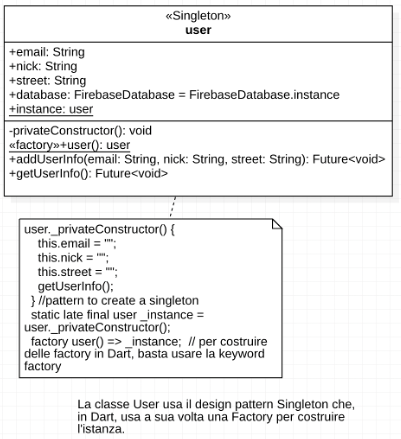
\includegraphics{Immagini/userClass.png} 

    \item -	Abstraction occurrence: questo design pattern è utilizzato nel caso dei singoli parrucchieri che vengono raggruppati nella classe HairStylists o nel caso delle prenotazioni e le classi per raggruppare le prenotazioni (StylistsBookings e ClientBookings), dove la relazione è composta da una classe che funge da Registro di tutte le occorrenze vere e proprie di una entità del mondo reale, che è rappresentata dalla seconda classe nella relazione.
    \item -	Façade: La classe AuthenticationService e la classe DatabaseService sono delle façade in quanto hanno il compito di offrire tutta una serie funzionalità (per il login e per gestione del database rispettivamente) usando i metodi di un'unica classe. I metodi offerti da queste classi si interfacciano direttamente con i servizi offerti di firebase, per i quali non sono noti i class diagram, di conseguenza queste associazioni non vengono descritte esplicitamente nel class diagram.
    \item -	Observer: la dinamica Observer-Observable è utilizzata con il meccanismo dei provider, che offrono dei metodi per rendere alcuni classi Observable e poter accedere a diversi valori e metodi e soprattutto ricevere notifiche di modifiche dal punto di vista di altre classi che diventano invece degli observer.   
\end{itemize} 

\subsection{Design methods}
Per sviluppare il design dell’applicazione si seguono le best practice e i design pattern consigliati per applicazioni dart con il framework Futter e, in più, considerando che si tratta di un software che usa un linguaggio di programmazione ad oggetti, si segue approssimativamente il design Method di Booch nel quale si parte per identificare le classi e oggetti, si procede a identificare il loro comportamento e attributi, successivamente si identificano le relazioni tra di loro e infine si fanno dei raffinamenti per procedere con una nuova iterazione del design. 
\\Nella pratica, l’applicazione di Booch al design specifico di questo applicativo coinvolge piccole fasi di implementazione dopo ogni singolo step, per informare meglio le scelte di design e valutare se le scelte fatte precedentemente sono fattibili nel contesto di Flutter e tenendo in conto le conoscenze iniziali limitate del team di development. 


\newpage
\section{Software Testing}
\subsubsection{IEEE928}
Questo tipo di documento si occupa di specificare e documentare come avviene la fase di testing
del progetto. Questo documento rappresenta anche il test plan. Siccome stiamo facendo un tipo di
sviluppo di software AGILE i test non vengono fatti alla fine ma vengono svolti assieme allo
sviluppo delle classi.
\\Viene svolto un tipo di sviluppo di tipo TDD in cui si scrivono le classi dei test in 
contemporanea (se non prima) delle classi che servono per il sito. Le fasi del testing sono le 
seguenti:
\begin{itemize}
    \item Preparation of tests 
    \item Running the  tests
    \item Completion of testing
\end{itemize} 

\subsubsection{Preparation of tests}
I test vengono fatti in contemporanea allo sviluppo delle classi, talvolta per alcune classi
sono stati fatti prima i test pensando poi alle classi che sarebbero state implementate successivamente.
I test per le classi in dart vengono scritti anche loro in linguaggio dart ed eseguiti tramite Junit.
\\Per quanto riguarda il testing di flutter si utilizza la funzione testWidgets che si importa 
dal pacchetto $flutter_test$ e permette di fare i test sulla web app.
\\Per garantire la CI (continuos integration) si utilizzerà Travis CI con i test che partiranno ad
ogni git e ogni 24 ore.
\\I test tenderanno ad essere il più possibile di tipo coverage in quanto si cercerà di coprire 
il più possibile i casi di test.
\\I test di Travis partono ogni 24 h sul main e ogni git su un branch specifico porta all'esecuzione 
del test in background su Travis. Ad ogni test viene fatta in automatico anche una build che permette
di vedere se ci sono eventuali errori diortografia all'interno del codice.
\\L'unico problema di Travis CI è che flutter non è supportato e non gestisce gli import correttamente e quindi è stato necessario importare (copiando) le classi che 
servivano per il testing.
\\L'interfaccia di Travis è la seguente:
\\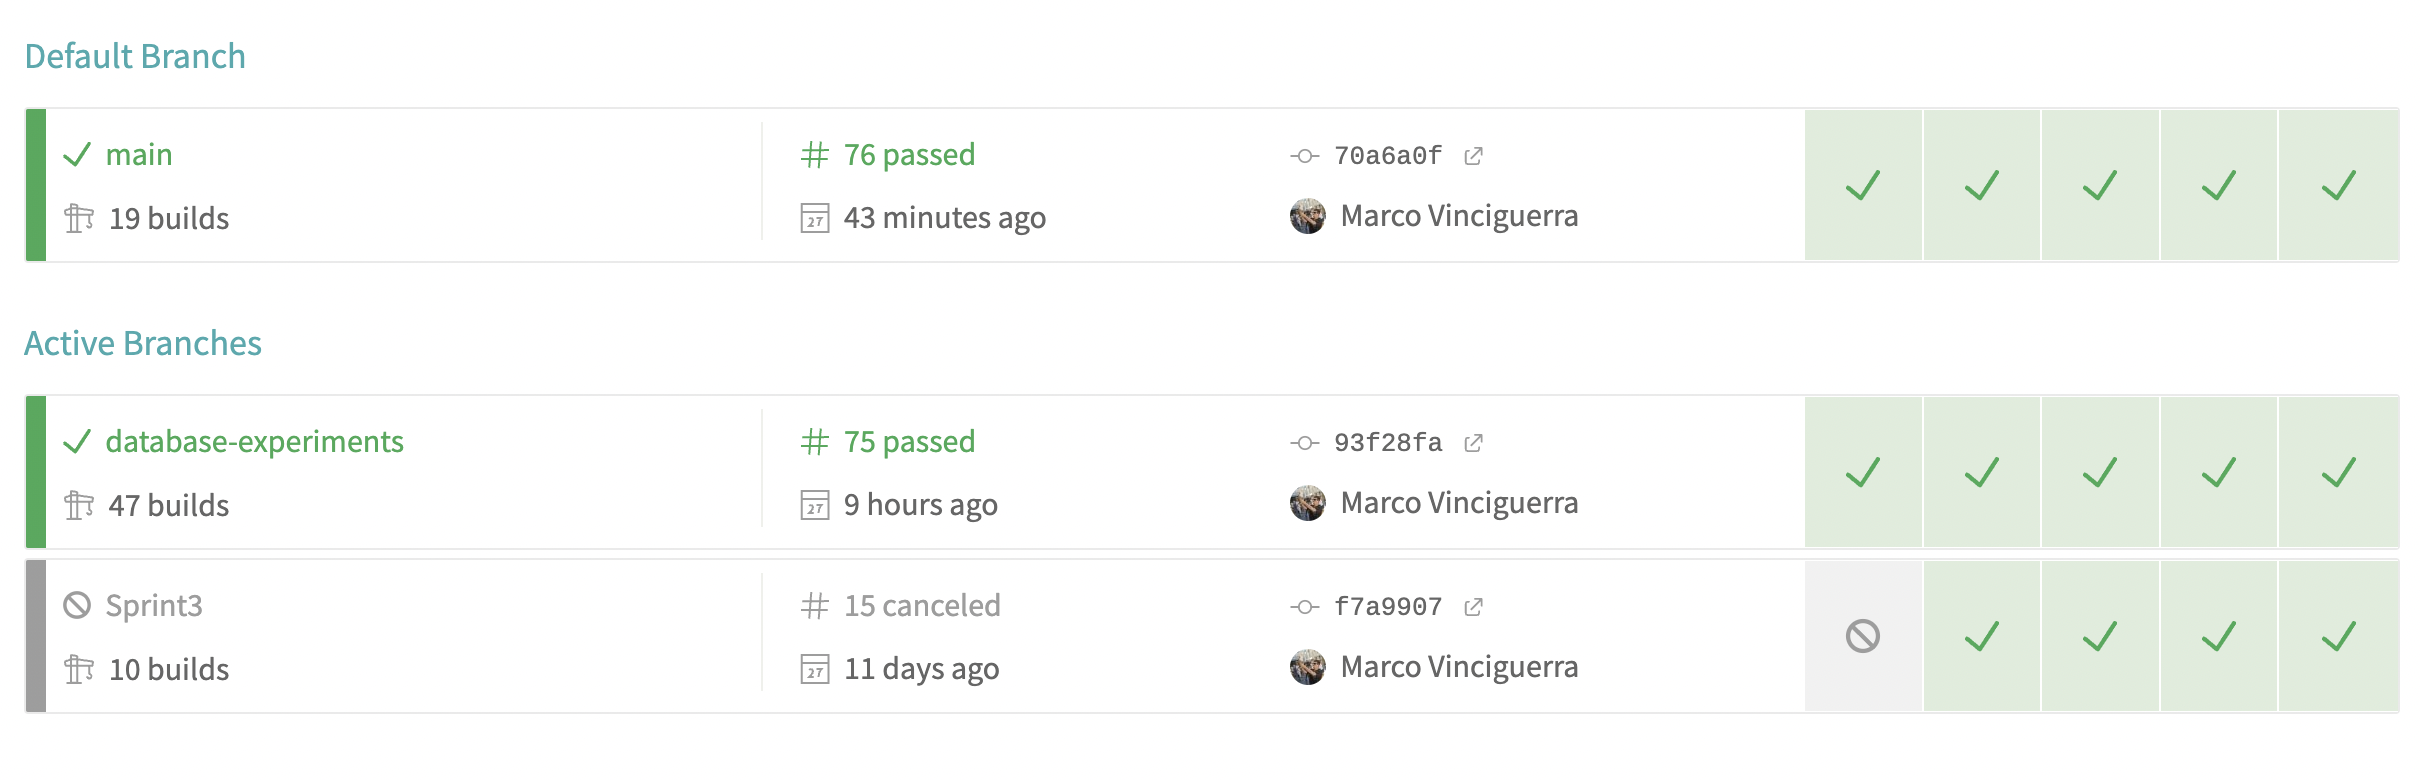
\includegraphics[scale = 0.25]{"Immagini/Travis.PNG"}
\\E' stato fatto anche il firrebase testing per vedere se l'applicazione funziona correttamente
sui dispositivi mobile.
\\In questo tipo di test sono stati presi diversi tipi di cellulari e installato in modo automatico 
l'apk e l'applicazione è stata testata per vedere se girasse in modo corretto.
\\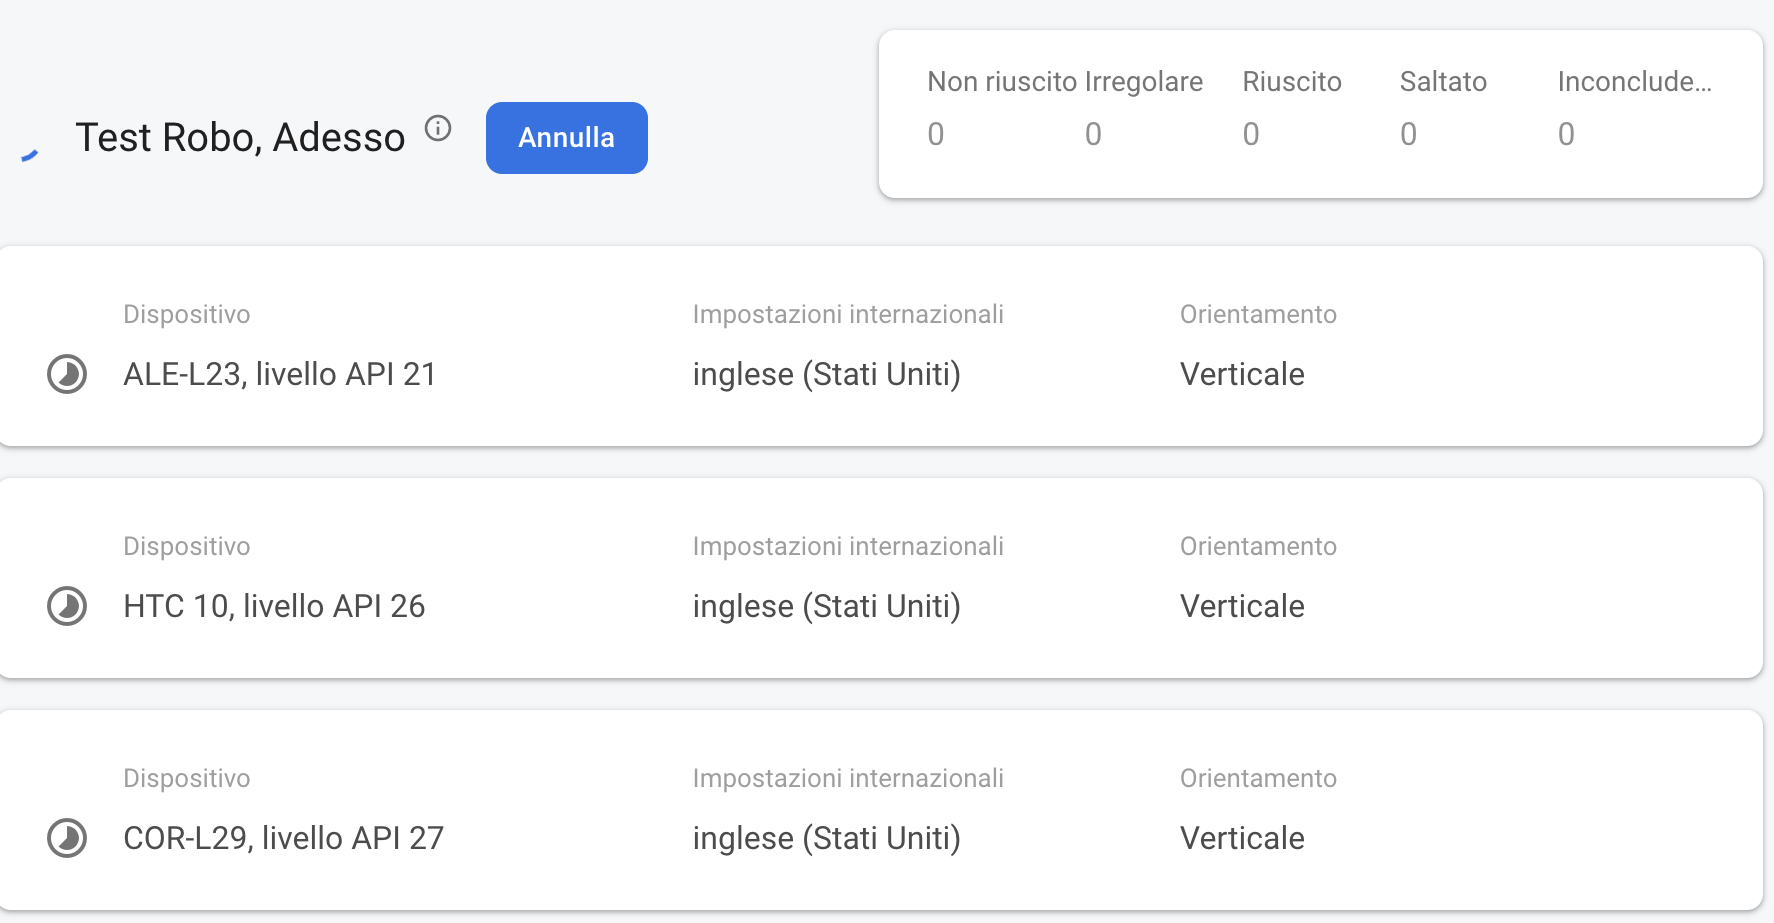
\includegraphics[scale = 0.45]{"Immagini/Firebase_testing.PNG"}
\\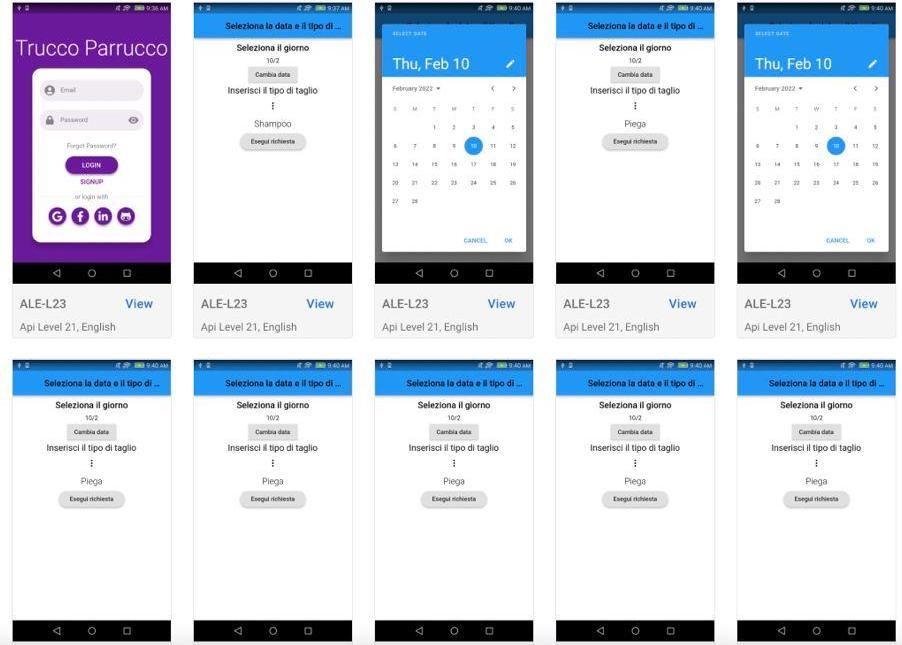
\includegraphics[scale = 0.50]{Immagini/firebaseTesting.jpg}

All'interno del progetto flutter vengono utilizzate 2 classi differenti che si occupano dello 
sviluppo del testing, essi sono:
\begin{itemize}
    \item $UnitTest.dart$: per fare unit testing
    \item $WidgetTest.dart$: per fare i test delle widget
\end{itemize}

\subsubsection{Running the tests}
Una volta fatte le classi ed eseguiti i test si procede in modo iterativo a modificare il codice
finchè i test non danno tutti risultati positivi. 

\subsubsection{Completion of testing}
I dati expected sono inventati e ad ogni iterazione si commentano i risultati per capire 
se va tutto bene e se c'è qualcosa che non quadra.

\newpage
\section{Software Maintenance}
Siccome non sapevamo fin da principio come utilizzare Flutter e firebase abbiamo alternato momenti di forwading engeneering con momenti di reverese
engeneering in cui si è sistemata la documentazione in funzione del codice che è stato scritto (redocumentation) facendo così un processo
di round trip engineering.
\\Il refactoring è stato fatto alla fine per separare le classi di dart per la view e per il model in delle cartelle apposite.
\\Per quanto riguarda il refactoring sono stati utilizzati i tool che Visual code per eseguire il refactoring (come ad esempio 
la possibilità di wrappare le widget o cambiare a cascata il nome di una classe).
\\Alla fine del progetto sono state rimosse anche le classi e i metodi non utilizzati (dead code).
\\Ad esempio è stato utilizzato il wrapp per creare il container di un widget in dart nel seguente modo:

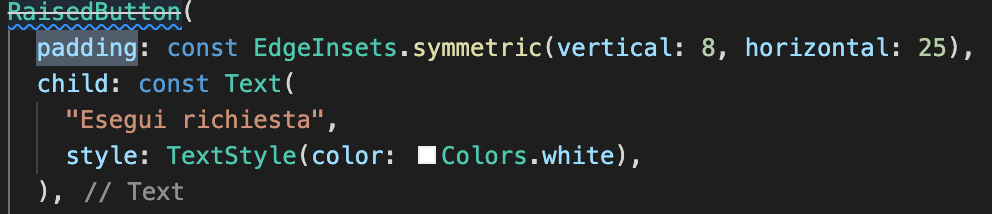
\includegraphics[scale = 0.25]{"Immagini/ref1.PNG"}
\\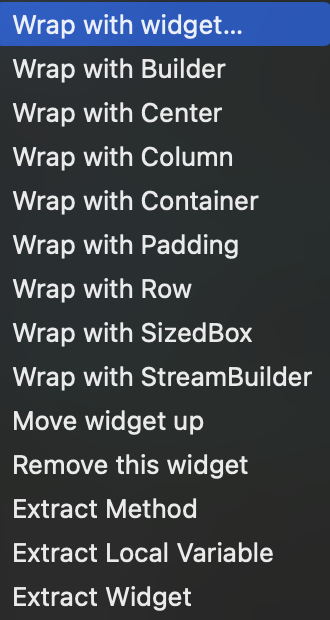
\includegraphics[scale = 0.25]{"Immagini/ref2.PNG"}

Un esempio di refactoring che è stato fatto è quello di aggiungere la parola const davanti agli elementi dei widget per aumentare le prestazioni

\end{document}
